\section{Discussion}

\begin{figure*}[!htbp]
\center
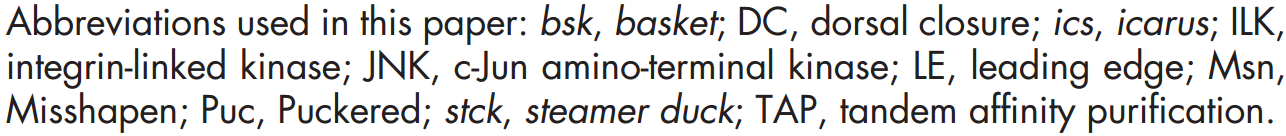
\includegraphics[width=0.6\textwidth]{alias}
\caption{A note containing explicit abbreviations from \newcite{kadrmas:2004}.}\label{fig:aliases}
\end{figure*}

This system, while productive, does not yet take maximal advantage of the information in the text. Future work and ongoing improvements are discussed next.

\subsection{Alias resolution}

Terminology is quite inconsistent between papers, because authors  often introduce name aliases for proteins or mutations such as ``E3 ligase BRAP (also referred to as IMP)''. These aliases will hold for the duration of the paper, but they generally do not appear in knowledge bases such as Uniprot \cite{uniprot}, which complicates resolution. In this case, the nonce equivalence of two names is informative for building models of interactions, in which the precise entity referred to must be known. In future work, we will implement patterns for the detection of these aliases when they are introduced, e.g., ``also referred to as''. Additionally, some papers contain a special section or note naming these aliases or abbreviations, as shown in Figure~\ref{fig:aliases}. Our coreference resolution system is currently being expanded to recognize text that marks two names equivalent in this way. 

%\todo{discuss more future work from your older analysis?}

\subsection{Informative ellipsis}

Because of the mechanistic nature of the events in this domain, authors may omit a great deal of information. For 
example, ellipsis, once reconstructed, can easily double the number of reactions detectable in a clause.

\begin{exe}
	\ex\label{ex:ellipsiswomod} The dephosphorylated {\it Axin} \underline{binds} $\beta$-catenin less efficiently than 
{\bf the phosphorylated form [of Axin} binds $\beta$-catenin].\footnote{Material between square brackets is added to 
complete the ellipsis and is not in the original text.}
	\ex	\begin{xlist}
		\ex[] {JNK-I revealed a stronger \underline{inhibitory} effect on IL-6 expression than the PKC-I [revealed an inhibitory effect on IL-6 expression].}\label{ex:verbalellipsis}
		\ex[*] {JNK-I revealed a stronger \underline{inhibitory} effect on IL-6 expression 
than [JNK-I revealed an inhibitory effect on] the PKC-I.}\label{ex:verbalellipsiswrong}
		\end{xlist}
\end{exe}

In example \ref{ex:ellipsiswomod}, proper understanding of the elided material allows us to capture the binding of 
phosphorylated Axin to beta-catenin as well as the negative regulation of dephosphorylation of Axin on the binding of 
Axin and $\beta$-catenin. To accomplish this, it is necessary to match the protein antecedent (Axin) but not the 
modification (dephosphorylation).

Similarly, the regulation of PKC-I on the IL-6 is captured only using ellipsis in example \ref{ex:verbalellipsis}. We must 
discount competing interpretations of the ellipsis such as that in example \ref{ex:verbalellipsiswrong}, which is a 
grammatically acceptable but factually incorrect alternative.

\subsection{Reference to latent entities}

The outputs of biochemical reactions are redundant with the reaction type and participants, so they are also often 
elided. For example, a (protein) binding reaction results in a (protein) complex made up of the participants in the 
binding. The complex may then be referred to without being explicitly named. This is essentially an anaphor without an 
explicit antecedent---a latent entity.

\begin{exe}
	\ex\label{ex:latent1} TGF$\beta$ signaling is initiated by the binding of TGF$\beta$ to TBRII. {\bf The [resulting] 
complex} [{\it TGF$\beta$:TBRII}] then \underline{recruits} TBRI.
\end{exe}

In example \ref{ex:latent1}, {\bf The complex} refers to {\it TGF$\beta$:TBRII}, the outcome of the binding described in the 
previous sentence. It is this complex that recruits (i.e., binds with) TBRI to form the complex TGF$\beta$:TBRII:TBRI.

This extension requires a model of the output of each event that has been found, work which is currently underway.

\section{Conclusion}

This work provides one of the first empirical measurements of the impact of entity and event coreference on large-scale event extraction in the biomedical domain. Furthermore, while prior work by \newcite{miwa2012coref} discusses the ideas of coreference in the biomedical domain, here we offer a concrete algorithm which leverages specific domain constraints.

This work was motivated by the observation that open-domain coreference resolution systems perform poorly in the biomedical domain because open-domain algorithms are insufficiently restrictive in this domain. To address this, we modified the sieve-based approach of \newcite{lee2013sieve} to infuse domain knowledge by: (i) removing open-domain sieves that do not transfer well to the biomedical domain; (ii) adding novel, domain-specific sieves, and (iii) constraining the remaining open-domain sieves with domain-specific restrictions that control which anaphors to resolve and which candidates to consider during the resolution process. 

We offer quantified results for a state-of-the-art event extraction system extended with the resulting coreference resolution approach, which show increased throughput at comparable precision when coreference resolution is used.

